\section*{A. Examples of Operations}

\begin{enumerate}

\item[1.]
\begin{equation}
a*b=\sqrt{|ab|} \text{, on the set } \mathbb{Q}
\end{equation}
This is not an operation because many roots are irrational

\item[2.]
\begin{equation}
a*b=\ln{b} \text{, on the set } \{x \in \mathbb{R} : x>0 \}
\end{equation}
This is an operation

\item[3.]
\begin{equation}
a*b \text{ is a root of the equation } x^2 - a^2b^2 = 0 \text{, on the set } \mathbb{R}
\end{equation}
This is not an operation because it is not uniquely defined for any $a\neq0$ $b\neq0$ because $x=a*b=\pm ab$

\item[4.]
\begin{equation}
\text{Subtraction, on the set } \mathbb{Z}
\end{equation}
This is an operation.

\item[5.]
\begin{equation}
\text{Subtraction, on the set } \{n \in \mathbb{Z} \geq 0 \}
\end{equation}
This is not an operation when $a-b \leq 0$

\item[6.]
\begin{equation}
a*b=|a-b| \text{, on the set } \{ n \in \mathbb{Z} \geq 0 \}
\end{equation}
This is an operation

\end{enumerate}

\section*{B. Properties of Operations}

\begin{enumerate}

\item[1.]
\begin{equation}
x*y=x+2y+4
\end{equation}

\begin{enumerate}

\item[i]
$y * x = y + 2x + 4 \neq x + 2y + 4$ \\
Not commutative

\item[ii]
$x*(y*z)=x(y+2z+4)=xy+2xz+4x \neq$ \\
$(x*y)*z=(x+2y+4)z=xz+2yz+4z$ \\
Not associative

\item[iii]
$x*e=x \text{ for } e: x*e=x+2e+4=x \text{; therefore } e=2 \neq$ \\
$e*y=y \text{ for } e: e*y=e+2y+4=y \text{; therefore } e=-y-4$ \\
Identity does not exist

\item[iiii]
Inverse can't exist without an identity

\end{enumerate}

\item[2.]
\begin{equation}
x*y=x+2y-xy
\end{equation}

\begin{enumerate}

\item[i]
$y*x=y+2x-yx \neq x+2y-xy=x*y$ \\
Not commutative

\item[ii]
$x*(y*z)=x*(y+2z-yz)=x+2(y+2z-yz)-x(y+2z-yz)=x+2y+4z-2yz-xy-2xz+xyz \neq$ \\
$(x*y)*z=(x+2y-xy)*z=(x+2y-xy)+2z-(x+2y-xy)z=x+2y-xy+2z-xz-2yz+xyz$ \\
Not associative

\item[iii]
$x*e=x+2e-xe=x \text{, therefore } e=0$ \\
$e*y=e+2y-ey=y \text{, therefore } e=\frac{-y}{1-y}$ \\
No identity

\item[iiii]
No inverse

\end{enumerate}

\item[3.]
\begin{equation}
x*y=|x+y|
\end{equation}

\begin{enumerate}

\item[i]
$y*x=|y+x|=|x+y|=x+y$ \\
Commutative

\item[ii]
$x*(y*z)=x*|y+z|=|x+|y+z||=$ \\
$(x*y)*z=|x+y|*z=||x+y|+z|$ \\
Not associative (for example let $x=2$, $y=-3$, $z=5$)

\item[iii]
$x*e=|x+e|=x$ \\
No identity

\item[iiii]
No inverse

\end{enumerate}

\item[4.]
\begin{equation}
x*y=|x-y|
\end{equation}

\begin{enumerate}

\item[i]
$y*x = |y-x| = |x-y| = x*y$ \\
Commutative

\item[ii]
$x*(y*z)=x*|y-z|=|x-|y-z||$ \\
$(x*y)*z=|x-y|*z=||x-y|-z|$ \\
Not associative (for example let $x=2$, $y=-3$, $z=5$)

\item[iii]
$x*e=|x-e|=x$ \\
No identity

\item[iiii]
No inverse

\end{enumerate}

\item[5.]
\begin{equation}
x*y=xy+1
\end{equation}

\begin{enumerate}

\item[i]
$y*x=yx+1=xy+1=x*y$ \\
Commutative

\item[ii]
$x*(y*z)=x*(yz+1)=x(yz+1)+1=xyz+x+1 \neq$ \\
$(x*y)*z=(xy+1)*z=(xy+1)z+1=xyz+z+1$ \\
Not associative

\item[iii]
$x*e=xe+1=x \text{, therefore } e=\frac{x-1}{x}$ \\
No identity

\item[iiii]
No inverse

\end{enumerate}

\item[6.]
\begin{equation}
x*y=max\{x,y\}
\end{equation}

\begin{enumerate}

\item[i]
$y*x=max\{y,x\}=max\{x,y\}=x*y$ \\
Commutative

\item[ii]
$x*(y*z)=x*max\{y,z\}=max\{x,max\{y,z\}\}=max\{x,y,z\}=$ \\
$(x*y)*z=max\{x,y\}*z=max\{max\{x,y\},z\}=max\{x,y,z\}$ \\
Associative

\item[iii]
$x*e=max\{x,e\}=x \text{, therefore } e=-\infty$ \\
No identity

\item[iiii]
No inverse

\end{enumerate}

\item[7.]
\begin{equation}
x*y=\frac{xy}{x+y+1} \text{(on the set of positive real numbers)}
\end{equation}

\begin{enumerate}

\item[i]
$y*x=\frac{yx}{y+x+1}=\frac{xy}{x+y+1}=x*y$ \\
Commutative

\item[ii]
\begin{multline}
x*(y*z)=x*\frac{yz}{y+z+1}=\frac{x\frac{yz}{y+z+1}}{x+\frac{yz}{y+z+1}+1}
= \frac{y z x}{1 + x + y + z + x y + x z + y z} =
\end{multline}
\begin{multline}
(x*y)*z=\frac{xy}{x+y+1}*z=\frac{\frac{xy}{x+y+1}z}{\frac{xy}{x+y+1}+z+1}
=\frac{x y z}{1 + x +y + z + x y + x z + y z}
\end{multline}
Associative

\item[iii]
$x*e=\frac{xe}{x+e+1}=x \text{, therefore } x=-1$ \\
No identity

\item[iiii]
No inverse

\end{enumerate}


\end{enumerate}

\section*{C. Operations on a Two-Element Set}

\begin{enumerate}

\item[1.]
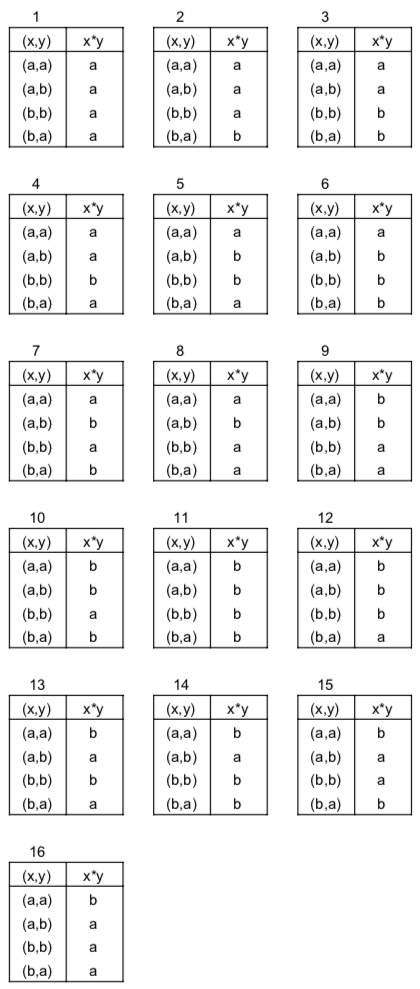
\includegraphics[scale=.48]{two-element-set}

\item[2.]
Commutative: 1, 4, 6, 7, 10, 11, 13, 16 \\
For all of these $(a,b) = (b,a)$

\item[3.]
Associative: 1, 3, 4, 5, 6, 7, 11, 13 \\
I used the following Clojure code to solve:
\begin{verbatim}
(def tables
  (for [aa ['a 'b]
        ab ['a 'b]
        bb ['a 'b]
        ba ['a 'b]]
    {['a 'a] aa
     ['a 'b] ab
     ['b 'b] bb
     ['b 'a] ba}))


(defn assoc?
  [table]
  (every? identity
          (for [x ['a 'b]
                y ['a 'b]
                z ['a 'b]]
            (= (table [(table [x y]) z])
               (table [x (table [y z])])))))

(->> tables
     (map (fn [table] [table (assoc? table)]))
     (filter second))
\end{verbatim}

\item[2.]
Have identity: 4, 6, 7, 13  \\
I used the following Clojure code to solve:
\begin{equation}
((a,a)=a \cap (a,b)=b \cap (b,a)=b) \cup ((b,b)=b  \cap (a,b)=a \cap (b,a)=a)
\end{equation}
\begin{verbatim}
(for [aa ['a 'b]
      ab ['a 'b]
      bb ['a 'b]
      ba ['a 'b]
      :when (or (and (= aa 'a)
                     (= ab 'b)
                     (= ba 'b))
                (and (= bb 'b)
                     (= ab 'a)
                     (= ba 'a)))]
  {['a 'a] aa
   ['a 'b] ab
   ['b 'b] bb
   ['b 'a] ba})
\end{verbatim}

\item[2.]
Have inverse: 7 and 13 \\
4 has identity $b$: there exists no $x$ where $a*x=b$\\
6 has identity $a$: there exists no $x$ where $b*x=a$\\
7 has identity $b$: $a*b=b=e$ and $b*a=b=e$\\
13 has identity $a$: $a*b=a=e$ and $b*a=a=e$\\

\end{enumerate}

\section*{D. Automata: The Algebra of Input/Output Sequences}

\begin{enumerate}

\item[1.]
Let $\boldsymbol{a}=a_{1}..a_{n}, \boldsymbol{b}=b_{1}..b_{m}, \boldsymbol{c}=c_{1}..c_{k}$ \\
$\boldsymbol{a}*(\boldsymbol{b}*\boldsymbol{c})=\boldsymbol{a}*(b_{1}..b_{m}c_{1}..c_{k})=a_{1}..a_{n}b_{1}..b_{m}c_{1}..c_{k}$ \\
$(\boldsymbol{a}*\boldsymbol{b})*\boldsymbol{c}=(a_{1}..a_{n}b_{1}..b_{m})*\boldsymbol{c}=a_{1}..a_{n}b_{1}..b_{m}c_{1}..c_{k}$

\item[2.]
Concatenation is not commutative because placing elements on to the beginning 
versus the end of a sequence leads to different sequences.

\item[3.]
Let $\boldsymbol{a}=a_{1}..a_{n}$ \\
$\boldsymbol{a} \lambda=\lambda \boldsymbol{a} = \boldsymbol{a}$ \\


\end{enumerate}